% Created by tikzDevice version 0.12.6 on 2026-07-06 23:55:44
% !TEX encoding = UTF-8 Unicode
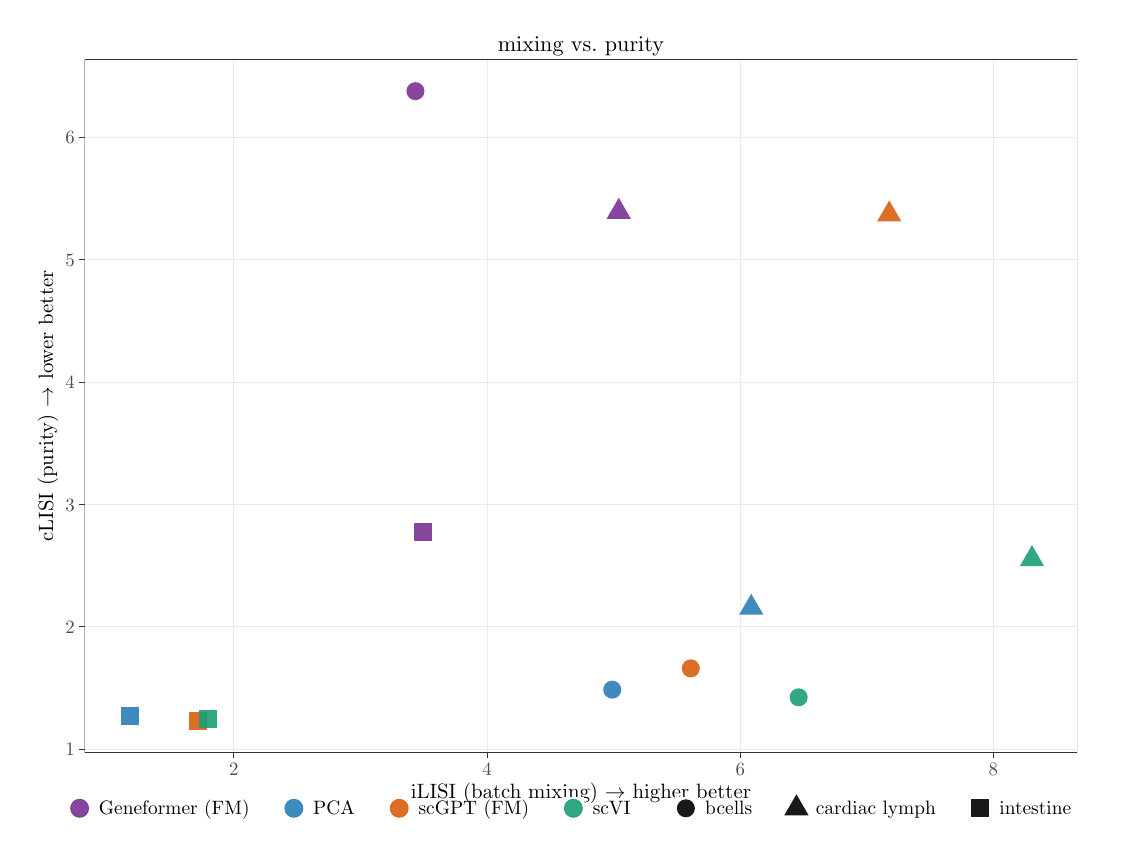
\begin{tikzpicture}[x=1pt,y=1pt]
\definecolor{fillColor}{RGB}{255,255,255}
\path[use as bounding box,fill=fillColor,fill opacity=0.00] (0,0) rectangle (385.20,289.08);
\begin{scope}
\path[clip] (  0.00,  0.00) rectangle (385.20,289.08);
\definecolor{drawColor}{RGB}{255,255,255}
\definecolor{fillColor}{RGB}{255,255,255}

\path[draw=drawColor,line width= 0.4pt,line join=round,line cap=round,fill=fillColor] (  0.00,  0.00) rectangle (385.20,289.08);
\end{scope}
\begin{scope}
\path[clip] ( 20.62, 27.23) rectangle (379.20,277.52);
\definecolor{fillColor}{RGB}{255,255,255}

\path[fill=fillColor] ( 20.62, 27.23) rectangle (379.20,277.52);
\definecolor{drawColor}{gray}{0.92}

\path[draw=drawColor,line width= 0.4pt,line join=round] ( 20.62, 28.33) --
	(379.20, 28.33);

\path[draw=drawColor,line width= 0.4pt,line join=round] ( 20.62, 72.54) --
	(379.20, 72.54);

\path[draw=drawColor,line width= 0.4pt,line join=round] ( 20.62,116.76) --
	(379.20,116.76);

\path[draw=drawColor,line width= 0.4pt,line join=round] ( 20.62,160.97) --
	(379.20,160.97);

\path[draw=drawColor,line width= 0.4pt,line join=round] ( 20.62,205.19) --
	(379.20,205.19);

\path[draw=drawColor,line width= 0.4pt,line join=round] ( 20.62,249.40) --
	(379.20,249.40);

\path[draw=drawColor,line width= 0.4pt,line join=round] ( 74.53, 27.23) --
	( 74.53,277.52);

\path[draw=drawColor,line width= 0.4pt,line join=round] (166.01, 27.23) --
	(166.01,277.52);

\path[draw=drawColor,line width= 0.4pt,line join=round] (257.48, 27.23) --
	(257.48,277.52);

\path[draw=drawColor,line width= 0.4pt,line join=round] (348.96, 27.23) --
	(348.96,277.52);
\definecolor{fillColor}{RGB}{217,95,14}

\path[fill=fillColor,fill opacity=0.90] (239.62, 57.57) circle (  3.26);
\definecolor{fillColor}{RGB}{123,50,148}

\path[fill=fillColor,fill opacity=0.90] (140.11,266.14) circle (  3.26);
\definecolor{fillColor}{RGB}{44,127,184}

\path[fill=fillColor,fill opacity=0.90] (211.23, 49.87) circle (  3.26);
\definecolor{fillColor}{RGB}{217,95,14}

\path[fill=fillColor,fill opacity=0.90] (311.32,226.66) --
	(315.71,219.06) --
	(306.93,219.06) --
	cycle;
\definecolor{fillColor}{RGB}{123,50,148}

\path[fill=fillColor,fill opacity=0.90] (213.58,227.62) --
	(217.97,220.02) --
	(209.20,220.02) --
	cycle;
\definecolor{fillColor}{RGB}{44,127,184}

\path[fill=fillColor,fill opacity=0.90] (261.46, 84.54) --
	(265.85, 76.94) --
	(257.07, 76.94) --
	cycle;
\definecolor{fillColor}{RGB}{217,95,14}

\path[fill=fillColor,fill opacity=0.90] ( 58.13, 35.35) --
	( 64.65, 35.35) --
	( 64.65, 41.86) --
	( 58.13, 41.86) --
	cycle;
\definecolor{fillColor}{RGB}{123,50,148}

\path[fill=fillColor,fill opacity=0.90] (139.67,103.68) --
	(146.19,103.68) --
	(146.19,110.20) --
	(139.67,110.20) --
	cycle;
\definecolor{fillColor}{RGB}{44,127,184}

\path[fill=fillColor,fill opacity=0.90] ( 33.66, 37.11) --
	( 40.18, 37.11) --
	( 40.18, 43.63) --
	( 33.66, 43.63) --
	cycle;
\definecolor{fillColor}{RGB}{27,158,119}

\path[fill=fillColor,fill opacity=0.90] (278.59, 47.11) circle (  3.26);

\path[fill=fillColor,fill opacity=0.90] (362.90,102.10) --
	(367.29, 94.50) --
	(358.51, 94.50) --
	cycle;

\path[fill=fillColor,fill opacity=0.90] ( 61.94, 36.11) --
	( 68.45, 36.11) --
	( 68.45, 42.62) --
	( 61.94, 42.62) --
	cycle;
\definecolor{drawColor}{gray}{0.20}

\path[draw=drawColor,line width= 0.4pt,line join=round,line cap=round] ( 20.62, 27.23) rectangle (379.20,277.52);
\end{scope}
\begin{scope}
\path[clip] (  0.00,  0.00) rectangle (385.20,289.08);
\definecolor{drawColor}{gray}{0.30}

\node[text=drawColor,anchor=base east,inner sep=0pt, outer sep=0pt, scale=  0.68] at ( 17.02, 25.98) {1};

\node[text=drawColor,anchor=base east,inner sep=0pt, outer sep=0pt, scale=  0.68] at ( 17.02, 70.20) {2};

\node[text=drawColor,anchor=base east,inner sep=0pt, outer sep=0pt, scale=  0.68] at ( 17.02,114.41) {3};

\node[text=drawColor,anchor=base east,inner sep=0pt, outer sep=0pt, scale=  0.68] at ( 17.02,158.63) {4};

\node[text=drawColor,anchor=base east,inner sep=0pt, outer sep=0pt, scale=  0.68] at ( 17.02,202.84) {5};

\node[text=drawColor,anchor=base east,inner sep=0pt, outer sep=0pt, scale=  0.68] at ( 17.02,247.06) {6};
\end{scope}
\begin{scope}
\path[clip] (  0.00,  0.00) rectangle (385.20,289.08);
\definecolor{drawColor}{gray}{0.20}

\path[draw=drawColor,line width= 0.4pt,line join=round] ( 18.62, 28.33) --
	( 20.62, 28.33);

\path[draw=drawColor,line width= 0.4pt,line join=round] ( 18.62, 72.54) --
	( 20.62, 72.54);

\path[draw=drawColor,line width= 0.4pt,line join=round] ( 18.62,116.76) --
	( 20.62,116.76);

\path[draw=drawColor,line width= 0.4pt,line join=round] ( 18.62,160.97) --
	( 20.62,160.97);

\path[draw=drawColor,line width= 0.4pt,line join=round] ( 18.62,205.19) --
	( 20.62,205.19);

\path[draw=drawColor,line width= 0.4pt,line join=round] ( 18.62,249.40) --
	( 20.62,249.40);
\end{scope}
\begin{scope}
\path[clip] (  0.00,  0.00) rectangle (385.20,289.08);
\definecolor{drawColor}{gray}{0.20}

\path[draw=drawColor,line width= 0.4pt,line join=round] ( 74.53, 25.23) --
	( 74.53, 27.23);

\path[draw=drawColor,line width= 0.4pt,line join=round] (166.01, 25.23) --
	(166.01, 27.23);

\path[draw=drawColor,line width= 0.4pt,line join=round] (257.48, 25.23) --
	(257.48, 27.23);

\path[draw=drawColor,line width= 0.4pt,line join=round] (348.96, 25.23) --
	(348.96, 27.23);
\end{scope}
\begin{scope}
\path[clip] (  0.00,  0.00) rectangle (385.20,289.08);
\definecolor{drawColor}{gray}{0.30}

\node[text=drawColor,anchor=base,inner sep=0pt, outer sep=0pt, scale=  0.68] at ( 74.53, 18.95) {2};

\node[text=drawColor,anchor=base,inner sep=0pt, outer sep=0pt, scale=  0.68] at (166.01, 18.95) {4};

\node[text=drawColor,anchor=base,inner sep=0pt, outer sep=0pt, scale=  0.68] at (257.48, 18.95) {6};

\node[text=drawColor,anchor=base,inner sep=0pt, outer sep=0pt, scale=  0.68] at (348.96, 18.95) {8};
\end{scope}
\begin{scope}
\path[clip] (  0.00,  0.00) rectangle (385.20,289.08);
\definecolor{drawColor}{RGB}{0,0,0}

\node[text=drawColor,anchor=base,inner sep=0pt, outer sep=0pt, scale=  0.75] at (199.91, 10.46) {iLISI (batch mixing) $\to$ higher better};
\end{scope}
\begin{scope}
\path[clip] (  0.00,  0.00) rectangle (385.20,289.08);
\definecolor{drawColor}{RGB}{0,0,0}

\node[text=drawColor,rotate= 90.00,anchor=base,inner sep=0pt, outer sep=0pt, scale=  0.75] at (  9.17,152.37) {cLISI (purity) $\to$ lower better};
\end{scope}
\begin{scope}
\path[clip] (  0.00,  0.00) rectangle (385.20,289.08);
\definecolor{fillColor}{RGB}{255,255,255}

\path[fill=fillColor] ( 14.77,  3.00) rectangle (225.84,  7.00);
\end{scope}
\begin{scope}
\path[clip] (  0.00,  0.00) rectangle (385.20,289.08);
\definecolor{fillColor}{RGB}{255,255,255}

\path[fill=fillColor] ( 14.77,  3.00) rectangle ( 22.77, 11.00);
\definecolor{drawColor}{RGB}{123,50,148}
\definecolor{fillColor}{RGB}{123,50,148}

\path[draw=drawColor,draw opacity=0.90,line width= 0.3pt,line join=round,line cap=round,fill=fillColor,fill opacity=0.90] ( 18.77,  7.00) circle (  3.26);
\end{scope}
\begin{scope}
\path[clip] (  0.00,  0.00) rectangle (385.20,289.08);
\definecolor{fillColor}{RGB}{255,255,255}

\path[fill=fillColor] ( 92.19,  3.00) rectangle (100.19, 11.00);
\definecolor{drawColor}{RGB}{44,127,184}
\definecolor{fillColor}{RGB}{44,127,184}

\path[draw=drawColor,draw opacity=0.90,line width= 0.3pt,line join=round,line cap=round,fill=fillColor,fill opacity=0.90] ( 96.19,  7.00) circle (  3.26);
\end{scope}
\begin{scope}
\path[clip] (  0.00,  0.00) rectangle (385.20,289.08);
\definecolor{fillColor}{RGB}{255,255,255}

\path[fill=fillColor] (130.25,  3.00) rectangle (138.25, 11.00);
\definecolor{drawColor}{RGB}{217,95,14}
\definecolor{fillColor}{RGB}{217,95,14}

\path[draw=drawColor,draw opacity=0.90,line width= 0.3pt,line join=round,line cap=round,fill=fillColor,fill opacity=0.90] (134.25,  7.00) circle (  3.26);
\end{scope}
\begin{scope}
\path[clip] (  0.00,  0.00) rectangle (385.20,289.08);
\definecolor{fillColor}{RGB}{255,255,255}

\path[fill=fillColor] (193.19,  3.00) rectangle (201.19, 11.00);
\definecolor{drawColor}{RGB}{27,158,119}
\definecolor{fillColor}{RGB}{27,158,119}

\path[draw=drawColor,draw opacity=0.90,line width= 0.3pt,line join=round,line cap=round,fill=fillColor,fill opacity=0.90] (197.19,  7.00) circle (  3.26);
\end{scope}
\begin{scope}
\path[clip] (  0.00,  0.00) rectangle (385.20,289.08);
\definecolor{drawColor}{RGB}{0,0,0}

\node[text=drawColor,anchor=base west,inner sep=0pt, outer sep=0pt, scale=  0.70] at ( 25.77,  4.59) {Geneformer (FM)};
\end{scope}
\begin{scope}
\path[clip] (  0.00,  0.00) rectangle (385.20,289.08);
\definecolor{drawColor}{RGB}{0,0,0}

\node[text=drawColor,anchor=base west,inner sep=0pt, outer sep=0pt, scale=  0.70] at (103.19,  4.59) {PCA};
\end{scope}
\begin{scope}
\path[clip] (  0.00,  0.00) rectangle (385.20,289.08);
\definecolor{drawColor}{RGB}{0,0,0}

\node[text=drawColor,anchor=base west,inner sep=0pt, outer sep=0pt, scale=  0.70] at (141.25,  4.59) {scGPT (FM)};
\end{scope}
\begin{scope}
\path[clip] (  0.00,  0.00) rectangle (385.20,289.08);
\definecolor{drawColor}{RGB}{0,0,0}

\node[text=drawColor,anchor=base west,inner sep=0pt, outer sep=0pt, scale=  0.70] at (204.19,  4.59) {scVI};
\end{scope}
\begin{scope}
\path[clip] (  0.00,  0.00) rectangle (385.20,289.08);
\definecolor{fillColor}{RGB}{255,255,255}

\path[fill=fillColor] (233.84,  3.00) rectangle (385.05,  7.00);
\end{scope}
\begin{scope}
\path[clip] (  0.00,  0.00) rectangle (385.20,289.08);
\definecolor{fillColor}{RGB}{255,255,255}

\path[fill=fillColor] (233.84,  3.00) rectangle (241.84, 11.00);
\definecolor{fillColor}{RGB}{0,0,0}

\path[fill=fillColor,fill opacity=0.90] (237.84,  7.00) circle (  3.26);
\end{scope}
\begin{scope}
\path[clip] (  0.00,  0.00) rectangle (385.20,289.08);
\definecolor{fillColor}{RGB}{255,255,255}

\path[fill=fillColor] (273.79,  3.00) rectangle (281.79, 11.00);
\definecolor{fillColor}{RGB}{0,0,0}

\path[fill=fillColor,fill opacity=0.90] (277.79, 12.07) --
	(282.18,  4.47) --
	(273.40,  4.47) --
	cycle;
\end{scope}
\begin{scope}
\path[clip] (  0.00,  0.00) rectangle (385.20,289.08);
\definecolor{fillColor}{RGB}{255,255,255}

\path[fill=fillColor] (340.16,  3.00) rectangle (348.16, 11.00);
\definecolor{fillColor}{RGB}{0,0,0}

\path[fill=fillColor,fill opacity=0.90] (340.90,  3.74) --
	(347.42,  3.74) --
	(347.42, 10.26) --
	(340.90, 10.26) --
	cycle;
\end{scope}
\begin{scope}
\path[clip] (  0.00,  0.00) rectangle (385.20,289.08);
\definecolor{drawColor}{RGB}{0,0,0}

\node[text=drawColor,anchor=base west,inner sep=0pt, outer sep=0pt, scale=  0.70] at (244.84,  4.59) {bcells};
\end{scope}
\begin{scope}
\path[clip] (  0.00,  0.00) rectangle (385.20,289.08);
\definecolor{drawColor}{RGB}{0,0,0}

\node[text=drawColor,anchor=base west,inner sep=0pt, outer sep=0pt, scale=  0.70] at (284.79,  4.59) {cardiac lymph};
\end{scope}
\begin{scope}
\path[clip] (  0.00,  0.00) rectangle (385.20,289.08);
\definecolor{drawColor}{RGB}{0,0,0}

\node[text=drawColor,anchor=base west,inner sep=0pt, outer sep=0pt, scale=  0.70] at (351.16,  4.59) {intestine};
\end{scope}
\begin{scope}
\path[clip] (  0.00,  0.00) rectangle (385.20,289.08);
\definecolor{drawColor}{RGB}{0,0,0}

\node[text=drawColor,anchor=base,inner sep=0pt, outer sep=0pt, scale=  0.80] at (199.91,280.57) {mixing vs.\ purity};
\end{scope}
\end{tikzpicture}
